\documentclass{standalone}
\usepackage[usenames,dvipsnames]{xcolor}

\usepackage{tikz}
\begin{document}
	\begin{tikzpicture}
		\node[anchor=south west,inner sep=0] (image) at (0,0) {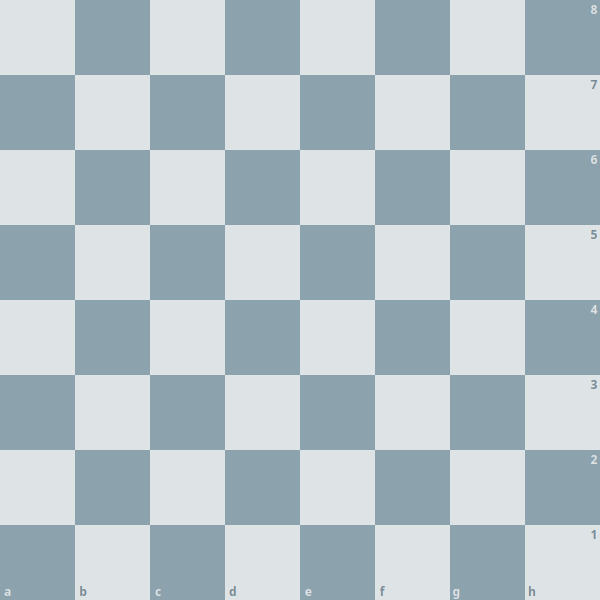
\includegraphics[width=\textwidth]{chess_board.png}};
		\begin{scope}[x={(image.south east)},y={(image.north west)}]
			%\draw[help lines,xstep=.1,ystep=.1] (0,0) grid (1,1);
			\draw[Red] (0.0625,0.0625) node {\Large $\mathbf{(1,1)}$};
			\draw[Red] (3*0.0625,11*0.0625) node {\Large $\mathbf{(2,6)}$};
			\fill[white, opacity=0.2, shift={(0.35,0.3)}]  (0,0) rectangle (0.35,0.15);
			\draw[draw=none, shift={(0.35,0.3)}] (0,0) rectangle (0.35,0.15) node[pos=0.5] {\parbox{3.5cm}{\Large \color{Red} \bf beide velden\\ zijn zwart}};
			\draw[Red, line width=2, -stealth] (0.35+0.35/2,0.3+0.15+0.01) -- (3*0.0625+0.05,11*0.0625-0.03);
			\draw[Red, line width=2, -stealth] (0.35+0.35/2,0.3-0.01) -- (0.0625+0.05,0.0625+0.03);
		\end{scope}
	\end{tikzpicture}
\end{document}